\RequirePackage{ifpdf}
\documentclass[letterpaper,landscape]{slides}
%\documentclass[letterpaper,portrait]{slides}
\usepackage{boxedminipage}
\usepackage{amsmath}
\usepackage{amssymb}

%\input /u/rhl/TeX/pdf.tex
\input pdf.tex

\newif\ifTalk\Talktrue		% We generating a talk, not printing
%\Talkfalse			% no; we're really printing

%\pagestyle{empty}
\setlength{\topmargin}{-1in}
\setlength{\textheight}{7.5in}
\setlength{\textwidth}{9in}
\setlength{\oddsidemargin}{0pt}
\setlength{\oddsidemargin}{0pt}

%\onlyslides{1-3,4,10-9999}
%\onlyslides{26-9999}

\begin{document}

\newcommand{\XXX}[1]{\textbf{XXX} #1}
\newcommand{\colour}[1]{\color{#1}}

\def\eq#1{\begin{equation} \color{blue} #1 \end{equation}}
\def\vx{{\bf x}}
\def\vv{{\bf v}}
\def\p{\partial}
\def\b#1{{\bf  #1}}
\def\p{\partial}
\def\th{^{th}}
\def\msun{{\rm\,M_\odot}}
\def\bnabla{{\bf\nabla}}
\def\dint{\int\!\!\!\int}
\def\d{{\rm d}}
\def\i{{\rm i}}
\def\ddt#1{{\rm{d} #1\over {\rm dt}}}
\def\ddtS#1{{\rm{d^2} #1\over {\rm dt^2}}}
%\lta and \gta produce > and < signs with twiddle underneath
\def\spose#1{\hbox to 0pt{#1\hss}}
\def\lta{\mathrel{\spose{\lower 3pt\hbox{$\mathchar"218$}}
     \raise 2.0pt\hbox{$\mathchar"13C$}}}
\def\gta{\mathrel{\spose{\lower 3pt\hbox{$\mathchar"218$}}
     \raise 2.0pt\hbox{$\mathchar"13E$}}}
\def\mspace{\hbox{\quad}}
\def\deffn#1{{\bf#1}}\def\eqs#1{equations \rf#1}






\newcount\itemCnt\itemCnt=0
\newcommand{\nitem}{%
  \global\advance\itemCnt by 1
  ~\vskip0cm\the\itemCnt.\qquad}

\definecolor{orange}{rgb}{1.0, 0.5, 0.0}
\definecolor{purple}{cmyk}{0.4, 0.8, 0.3, 0.0}


%%%%%%%%%%%%%%%%%%%%%%%%%%%%%%%%%%%
\newcommand{\onepic}[6]{%
\begin{slide}
     \begin{center}
        \begin{minipage}{#1in}
            {\large \color{blue} #6}
            \phantom{x} \vskip #2in
            \phantom{x} \hskip #3in
            {\scalebox{#4}{\includegraphics{#5}}}   
        \end{minipage}
     \end{center}
    \vfill
\end{slide}
}


%%%%%%%%%%%%%%%%%%%%%%%%%%%%%%%%%%%
\newcommand{\picslide}[7]{%
  \begin{slide}
     \begin{center}
        \begin{minipage}{#5in}
            \hskip #6in
            \hskip -1in
            {\scalebox{#4}{\includegraphics{#1.#2}}}
            \vskip #7in~
            {\large \color{blue} #3}
        \end{minipage}
     \end{center}
     \vfill
  \end{slide}
}
%%%%%%%%%%%%%%%%%%%%%%%%%%%%%%%%%%%
 

%%%%%%%%%%%%%%%%%%%%%%%%%%%%%%%%%%%
\newcommand{\Spicslide}[7]{%
  \begin{slide}
     \begin{center}
        \begin{minipage}{#5in}
            \vskip #6in
            \hskip #7in
            {\scalebox{#4}{\includegraphics{#1.#2}}}
        \end{minipage}
     \end{center}
     \vfill
  \end{slide}
}
%%%%%%%%%%%%%%%%%%%%%%%%%%%%%%%%%%%
 



%------------------------------------------------------------------------------

\begin{slide}

\phantom{x}
\vskip -2in
\begin{center}
\bfseries
{\large {\color{blue} Astr 511: Galaxies as galaxies}}
\end{center}

{\centerline {{\color{blue} 
Winter Quarter 2017, University of Washington}}}
{\centerline {{\color{blue} 
Mario Juri\'{c} \& \v{Z}eljko Ivezi\'{c} }}}

\vskip 1.6in

{\centerline {\Large {\color{red}      Lecture 7:             }}}
\vskip 0.2in 
{\centerline {\huge {\color{blue} Dynamics II: Galaxies as }}}
\vskip 0.1in
{\centerline {\huge {\color{blue} Collisonless Systems }}}

\vfill
\end{slide}
%------------------------------------------------------------------------------

%------------------------------------------------------------------------------
\begin{slide}
\begin{center}
{\large \color{red} Modeling Galaxies }
\end{center}

In the previous lecture we learned how to qualitatively (and quantitatively)
understand observed properties of galaxies by considering some (static)
potentials and orbits that those potentials admit.

But we haven't tackled the more difficult problem: how does one find
self-consistent, equilibrium, solutions of the Poisson equation equation
$\nabla^2 \Phi = 4 \pi G \rho$, that we can compare to the data? How do we
``build'' a model of a galaxy?

This is the problem we'll turn to in this lecture. But first...

\vfill
\end{slide}

%------------------------------------------------------------------------------
\begin{slide}
\begin{center}
{\large \color{red} Galaxies in Continuum Approximation }
\end{center}

How do we understand the internal dynamics of galaxies?  We could go back to
basic, and treat them as N-body systems consisting of (at least) $N \sim
10^{10}$ objects.  That will, however, be quickly revealed as impractical (to
put it mildly...).

Taking a hint from fluid dynamics, we try a different approach: could we
consider them as made up from a smooth, continous, fluid instead?  That is,
how accurately can we approximate a galaxy of $N$ identical stars of mass
$m$ as {\bf a smooth density distribution plus a gravitational field?}

{\em To answer this question, let's observe the motion of an individual star as its
orbit carries it once across the galaxy. Let's find an order-of-magnitude
estimate of the difference between the actual velocity of this star, and the
velocity that it would have had if the masses of other stars were smoothly
distributed.}

\vfill
\end{slide}



%------------------------------------------------------------------------------
\begin{slide}
\begin{center}
{\large \color{red} Two-body Scattering }
\end{center}

\begin{center}
\vskip -0.0in
\scalebox{0.5}{\hskip 0.0in 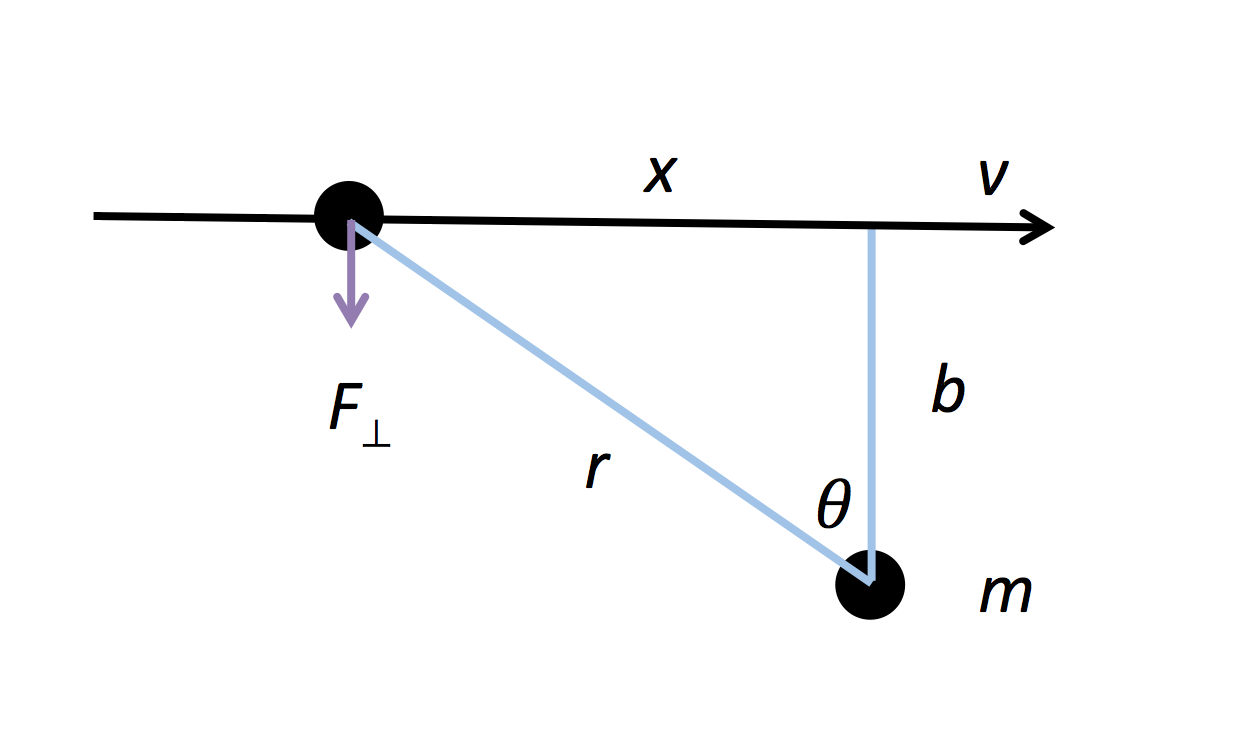
\includegraphics{figures/scattering.png}}
\end{center}

Consider the situation above, where a {\bf subject star} (top) scatters off
of a {\bf field star} (bottom) with an {\bf impact parameter} $b$ (the
distance of closes approach).  Assume
the deflection is {\em small} (i.e., the trajectory roughly remains to be a
straight line).  To an order of magnitude, the deflection $\delta v$ will be
given by:

\eq{
	\delta v = F_\perp \times \delta t_{encounter} = 
	   \left(\frac{G m}{b^2}\right) \times \left(\frac{2 b}{v}\right) =
	   \frac{2 G m}{b v}
}

\vfill
\end{slide}


%------------------------------------------------------------------------------
\begin{slide}
\begin{center}
{\large \color{red} Two-body Scattering }
\end{center}

\begin{center}
\vskip -0.0in
\scalebox{0.5}{\hskip 0.0in 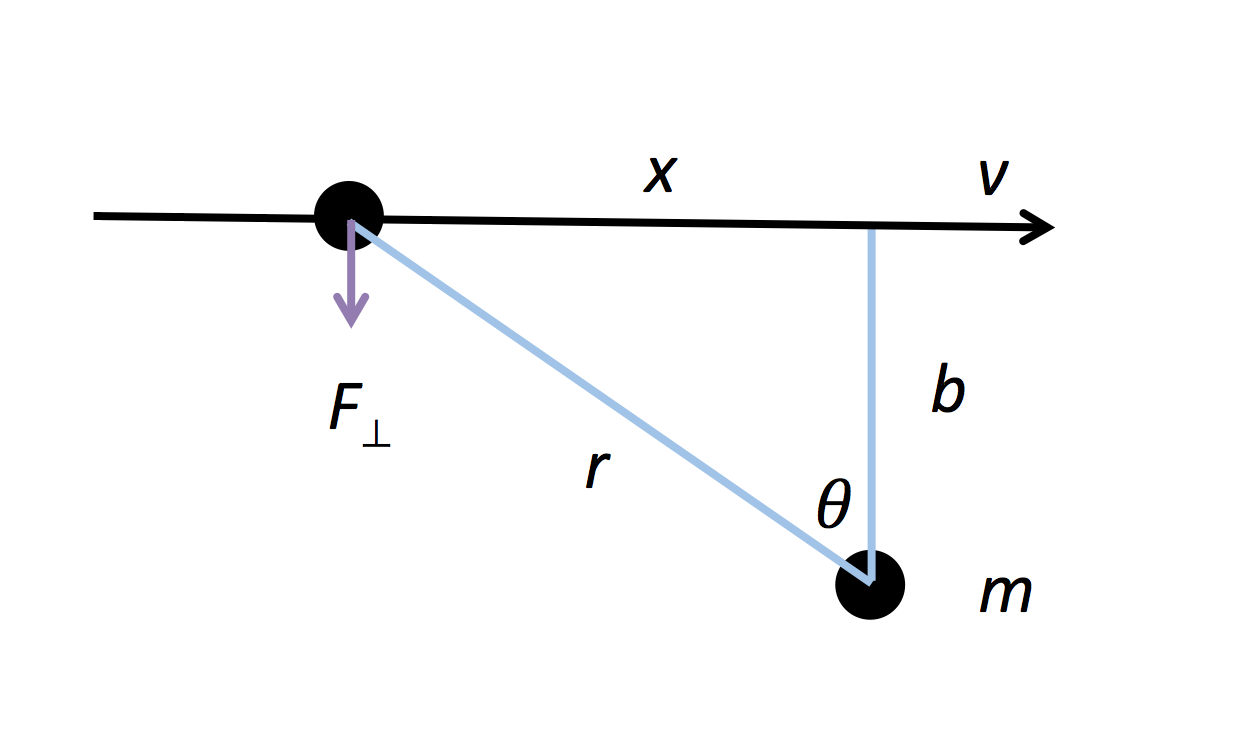
\includegraphics{figures/scattering.png}}
\end{center}

When does this line of reasoning break down? Definitely when $\delta v
\approx v$. What does that equate to in terms of the impact parameter $b$?
\eq{
	b \lesssim b_{\rm min} \equiv \frac{2 G m}{v^2} \eqsim {R \over N}
}
where the last equality comes from $v^2 = \frac{G M}{R} = \frac{ G N m}{R}$,
the circular velocity at radius $R$.

\vfill
\end{slide}


%------------------------------------------------------------------------------
\begin{slide}
\begin{center}
{\large \color{red} Galaxies as Collisionless Systems }
\end{center}

What is $b_{\rm min}$ for the Milky Way? Plugging in $R = 10$kpc and $N=10^{10}$
we get:
\eq{
	b_{\rm min,MW} \simeq = 3 \times 10^7 {\rm m} \simeq 50 R_\odot
}
Your intuition already tells you this kind of encounter will be infrequent.
How infrequent?

If we consider the probability of a disk of cross section
$4 \pi b_{\rm min, MW}^2$ to experience a collision while crossing a spherical
galaxy with density $n = \frac{3 N}{4 \pi R^3}$, we find:
\eq{
	t_{scatter} \simeq \left(\frac{R}{b_{\rm min}}\right)\frac{t_{cross}}{N} = N t_{cross}
}
where $t_{cross} \simeq 50$Myr and $N \approx 10^{10}$. Therefore,  {\bf the
Milky Way is a {\em collisionless system}}. I.e., stars almost never
``collide'' (strongly scatter) in the MW!

\vfill
\end{slide}



%------------------------------------------------------------------------------
\begin{slide}
\begin{center}
{\large \color{red} Relaxation time }
\end{center}

How long does it take for a star's velocity to change appreciably due to the
two-body scattering it experiences?

As the star crosses, these interactions accumulate. They do not change the
mean velocity (i.e. $\Delta v_\perp = 0$), but only the variance $(\Delta
v_\perp)^2$. In one crossing, a star experiences:
\eq{
	\delta n = \left(\frac{N}{\pi R^2}\right) \left(2 \pi b \right)db = \frac{2 N}{R^2} b db
}
encounters with impact parameters between $b$ and $b + db$. The total change
in $(\Delta v_\perp)^2$ is therefore:
\eq{
	\int d (\Delta v_\perp)^2 =
	\int_{b_{\rm min}}^{R} \left(\frac{2 G m}{b v}\right)^2 \frac{2 N b}{R^2} db =
	8 N \left(\frac{G m}{R v}\right)^2 \int_{b_{\rm min}}^{R} \frac{db}{b}
}
\eq{
	(\Delta v_\perp)^2 = 8 N \left(\frac{G m}{R v}\right)^2 \ln \Lambda
}
where $\ln \Lambda = \ln {R \over b_{\rm min}} = \ln N$ is know as the {\bf Coulomb logarithm}.

\vfill
\end{slide}


%------------------------------------------------------------------------------
\begin{slide}
\begin{center}
{\large \color{red} Relaxation time }
\end{center}

So, putting it all together, we have:
\eq{
	(\Delta v_\perp)^2 = \frac{8 \ln N}{N} \left(\frac{G N m}{R}\right)^2 \frac{1}{v^2} = \frac{8 \ln N}{N} v^2
}
\eq{
	\frac{(\Delta v_\perp)^2}{v^2} \eqsim 10 \frac{\ln N}{N}
}
meaning that it takes about $\sim .1 \times N / ln N$ crossings for $(\Delta
v_\perp)^2$ to become comparable to $v^2$. Expressed in terms of timescales:

\eq{
	t_{\rm relax} = \frac{N}{10 \ln N} t_{\rm cross}
}

where $t_{\rm relax}$ is the {\bf relaxation time} -- the time it takes the
system to ``forget'' its initial conditions.

\vfill
\end{slide}

%------------------------------------------------------------------------------
\begin{slide}
\begin{center}
{\large \color{red} Relaxation time }
\end{center}

Relaxation time:
\eq{
	t_{\rm relax} = \frac{N}{10 \ln N} t_{\rm cross} = \frac{1}{10 \ln N} t_{\rm scatter}
}
\vskip -1em
Plugging in the numbers for the Milky Way, we find that
$t_{\rm relax} \approx 2 \times 10^6$~Gyr, {\bf i.e., the Milky Way (and galaxies in general) 
are not relaxed systems}. In other words, {\bf global galaxy properties that we observe are 
largely a consequence of their formation}.

N.b.: typically, in collisionless systems we have:
\eq{
	t_{\rm cross} \ll t_H \eqsim t_{\rm form} \ll t_{relax} \ll t_{scatter} \ll t_{coll}
}

\vfill
\end{slide}


%------------------------------------------------------------------------------
\begin{slide}
\vskip 4.5in
\begin{center}
{\large \color{red} 
                  Equilibria of Colisionless Systems   }
\end{center}

\vskip 3.8in

\begin{flushright}
{ \tiny - Binney \& Tremaine, Chapter 4. } \\
\end{flushright}

\end{slide}


%------------------------------------------------------------------------------
\begin{slide}
\begin{center}
{\large \color{red} 
        The Distribution Function (DF) }
\end{center}

The positions and motions of stars can be described by a 
{\color{blue} phase-space distribution function $f(\vx, \vv, t)$} (aka
the phase-space number density).

The {\bf distribution function (DF)} fully encodes the state of a 
dynamical system (i.e., we know where all parcels of matter are, and how
they're moving).

For example, the density distribution is an integral over the velocities:
\eq{
	\rho = \int f(x, v, t) d{\bf v}
}
etc.

\vfill
\end{slide}


%------------------------------------------------------------------------------
\begin{slide}
\begin{center}
{\large \color{red} 
        Time evolution of a collisionless system }
\end{center}

The time evolution of $f(\vx, \vv, t)$ is governed by Newtonian dynamics:
\eq{
	\nabla^2 \Phi = 4 \pi G \rho
}
Assuming that stars can be neither created nor destroyed, the {\bf continuity
equation}:
\eq{
  { \frac{\p f}{\p t} + \nabla \cdot (f {\bf v}) = 0 }
}
can be applied to $f(\vx, \vv, t)$. In six-dimensional space
described by $w_i=(\vx, \vv) = (x_1, x_2, x_3, v_1, v_2, v_3)$, 
\eq{
  {\p f(\b w, t) \over \p t} + \sum_{i=1}^6 {\p \left( f(\b w, t) \dot w_i \right) \over \p w_i} = 0.
}


\vfill
\end{slide}



%------------------------------------------------------------------------------
\begin{slide}
\begin{center}
{\large \color{red} 
                    The collisonless Boltzmann Equation      }
\end{center}

\eq{
 {\p (f \dot w_i) \over \p w_i} = \dot w_i {\p f  \over \p w_i} + f {\p \dot w_i  \over \p w_i}
}

Note that the last term is either $(\p v_i / \p x_i)$, or $(\p \dot v_i / \p v_i)$. 

{\color{red} This term is always zero:} in the first case because $v_i$ and $x_i$ are independent coordinates, 
and in the second case because $\dot v_i = - (\p \Phi / \p x_i)$, and $\Phi$ does not depend 
on velocity (because it's gravitational potential). Hence, 

\eq{
   {\p f(\b w, t) \over \p t} + \sum_{i=1}^6 \dot w_i {\p f(\b w, t) \over \p w_i} = 0.  
}


\vfill
\end{slide}




%------------------------------------------------------------------------------
\begin{slide}
\begin{center}
{\large \color{red} 
                    The collisonless Boltzmann Equation  (CBE)    }
\end{center}

We therefore obtain the {\bf collisionless Boltzmann Equation}:

\eq{
   {\p f \over \p t} + {\bf x} {\p f \over \p {\bf x}} + {\bf v} {\p f \over \p {\bf v}} = 0
 \mspace {\rm or\, compactly} \mspace {df \over dt} = 0
}

This is the equation of motion of self-gravitating collisionless fluid. In other forms:

\eq{
{\p f \over \p t} + \sum_{i=1}^3 \left[ v_i {\p f \over \p x_i} - {\p \Phi \over \p x_i} {\p f \over \p v_i} \right]=0 
}

\eq{
    {\p f \over \p t} + \vv \nabla f = \nabla \Phi {\p f \over \p \vv}
}


\vfill
\end{slide}


%------------------------------------------------------------------------------
\begin{slide}
\begin{center}
{\large \color{red} 
                    The collisonless Boltzmann Equation  (CBE)    }
\end{center}


The last (vector) notation is the most useful one for expressing
the collisonless Boltzmann equation in arbitrary coordinate systems

The CBE is very difficult to solve directly (and hence not terribly useful
from that standpoint), but forms a) the basis for deriving {\color{blue} the
Jeans equations}, and b) the starting point for N-body methods
({\color{blue} N-body codes are essentially Monte-Carlo solvers of the
CBE}).

A side note: the radiative transfer equation is also a special case
of the general Boltzmann Equation (in the limit that all particles
move at the same speed). 


\vfill
\end{slide}





%------------------------------------------------------------------------------
\begin{slide}
\begin{center}
{\large \color{red} 
                    The Moment Equations     }
\end{center}

Some insights can be obtained by integrating the CBE multiplied by powers 
of the coordinates and/or velocities. By doing so we will end up
with differential equations for the evolution of various {\bf moments} of
the distribution function.

For example, let us integrate the CBE over all velocities:

\eq{
\int {\p f \over \p t} \d^3 \b v + \int v_i {\p f \over \p x_i} \d^3
\b v - {\p \Phi \over \p x_i} \int { \p f \over \p v_i} \d^3 \b v = 0.
\label{vmom}
}

\vfill
\end{slide}


%------------------------------------------------------------------------------
\begin{slide}
\begin{center}
{\large \color{red} 
                    The Moment Equations     }
\end{center}

For example, let us integrate the CBE over all velocities:
\eq{
\int {\p f \over \p t} \d^3 \b v + \int v_i {\p f \over \p x_i} \d^3
\b v - {\p \Phi \over \p x_i} \int { \p f \over \p v_i} \d^3 \b v = 0.
\label{vmom}
}

How do we evaluate these integrals? Two rules: 
\begin{enumerate}
\item Derivative wrt $\vx$, or a function of $\vx$, can be taken out of the
integral as {\bf v} and {\bf x} are independent, and
\item Let us introduce the notation 
\eq{
     \int g(\vv) f \d^3 \b v \, = \,\, <g> \int f \d^3 \b v 
}
where
\eq{
      \nu(\vx) = \int f \d^3 \b v 
}
is the number density as a function of position.
\end{enumerate}

\vfill
\end{slide}


%------------------------------------------------------------------------------
\begin{slide}
\begin{center}
{\large \color{red} 
                    The Moment Equations     }
\end{center}

Then
\eq{
\int {\p f \over \p t} \d^3 \b v + \int v_i {\p f \over \p x_i} \d^3
\b v - {\p \Phi \over \p x_i} \int { \p f \over \p v_i} \d^3 \b v = 0.
\label{vmom}
}
with
\eq{
\overline{v}_i \equiv { 1 \over \nu} \int f v_i \d^3 \b v,
}
becomes
\eq{
{\p \nu \over \p t} + { \p (\nu \overline{v}_i) \over \p x_i} = 0. \label{cont}
}
This is just the continuity equation for the stellar number density in real
space!

More interesting results are obtained by multiplying the CBE with higher powers
of $\vv$. 
\vfill
\end{slide}


%------------------------------------------------------------------------------
\begin{slide}
\begin{center}
{\large \color{red} 
                    The Moment Equations     }
\end{center}

E.g. take the first velocity moment of the CBE. Then
\eq{
\int {\p f \over \p t} \d^3 \b v + \int v_i {\p f \over \p x_i} \d^3
\b v - {\p \Phi \over \p x_i} \int { \p f \over \p v_i} \d^3 \b v = 0.
}
becomes
\eq{
{\p \over \p t} \int f v_j \d^3 \b v + \int v_i v_j {\p f \over \p x_i} \d^3
\b v - {\p \Phi \over \p x_i} \int v_j { \p f \over \p v_i} \d^3 \b v = 0.
\label{v1mom}
}
We can use the divergence theorem to manipulate the last term
\eq{
\int v_j { \p f \over \p v_i} \d^3 \b v = - \int {\p v_j \over \p v_i}
f \d^3 \b v = -\int \delta_{ij} f \d^3 \b v = -\delta_{ij}\nu,
\label{vmom2}
}
Note that 
\eq{
  v_j { \p f \over \p v_i} = -f { \p v_j \over \p v_i} + { \p (v_j f) \over \p v_i}
}
and the last term must be 0 when the integration surface is expendend to 
infinity (where $f$ must vanish).
\vfill
\end{slide}

%------------------------------------------------------------------------------
\begin{slide}
\begin{center}
{\large \color{red} 
                    The Moment Equations     }
\end{center}
Eq.(\ref{vmom2}) can be substituted into (\ref{v1mom}) giving
\eq{
{\p (\nu \overline{v_j}) \over \p t} + {\p (\nu \overline{v_i v_j})
\over \p x_i} + \nu {\p \Phi \over \p x_j} = 0,
}
where
\eq{
    \overline{v_i v_j} \equiv {1 \over \nu} \int v_i v_j f\d^3 \b v.
}
This is an equation of momentum conservation. 


\vfill
\end{slide}

%------------------------------------------------------------------------------
\begin{slide}
\begin{center}
{\large \color{red} 
                    The Moment Equations     }
\end{center}


Each velocity can be expressed as a sum of the mean value (aka streaming
motion) and the so-called peculiar velocity
\eq{
                   v_i = \overline{v_i} + w_i
}
where $\overline{w_i}=0$ by definition. Then
\eq{
\sigma^2_{ij} \equiv \overline{w_i w_j} =  
\overline{( v_i - \overline{v}_i)(v_j -
\overline{v}_j)} = \overline{v_i v_j} - \overline{v}_i \overline{v}_j.
}

At each point $\b x$ the symmetric tensor $\b\sigma^2$ defines an
ellipsoid whose principal axes run parallel to $\b\sigma^2$'s
eigenvectors and whose semi-axes are proportional to the square roots
of $\b\sigma^2$'s eigenvalues.  This is called the {\bf velocity
ellipsoid} at $\b x$. We have encountered it when discussing the LOSVD in
Lecture 5, and we'll encounter it again when we examine the kinematics
of the Milky Way.

\vfill
\end{slide}



%------------------------------------------------------------------------------
\begin{slide}
\begin{center}
{\large \color{red} 
                    The Jeans Equations   }
\end{center}

Taken together, the continuity equation:
\eq{
{\p \nu \over \p t} + { \p (\nu \overline{v}_i) \over \p x_i} = 0. \label{cont}
}
and the momentum equation
\eq{
\nu {\p \overline{v_j} \over \p t} + \nu \overline{v_i} {\p \overline{v_j} \over \p x_i} 
  = -\nu {\p \Phi \over \p x_j} - {\p (\nu \sigma^2_{ij}) \over \p x_i} 
}
are commonly know as the {\bf Jeans Equations}. They are analogous to Euler equations
of fluid dynamics. The term $-\nu \sigma^2_{ij}$ is a {\bf stress tensor} -- it describes 
anisotropic pressure.

Note that {\bf the system is not closed} (like it is in gases): there is no 
``equation of state''! The multiplication by higher powers of $\vv$ doesn't
help -- need an {\it ansatz}. In practice one
assumes a particular form for $\sigma^2_{ij}$, e.g. for isotropic velocity
dispersion $\sigma^2_{ij} = \sigma^2 \delta_{ij}$

\vfill
\end{slide}



%------------------------------------------------------------------------------
\begin{slide}
\begin{center}
{\large \color{red} 
                    The Jeans Equations   }
\end{center}

{\bf Specialization for an axially symmetric system:}

First express the CBE in cylindrical coordinates 
\eq{
{\p f \over \p t} 
+ \dot R {\p f \over \p R}   
+ \dot \phi {\p f \over \p \phi}   
+ \dot z {\p f \over \p z} 
+ \dot v_R {\p f \over \p v_R} 
+ \dot v_\phi {\p f \over \p v_\phi} 
+ \dot v_z {\p f \over \p v_z} = 0
}

With $\dot R \equiv v_R$, $\dot \phi \equiv v_\phi/R$, and $\dot z \equiv v_z$, and
\eq{
    \dot v_R = - {\p \Phi \over \p R} + {v_\phi^2 \over R}
}
\eq{
    \dot v_\phi = - {1 \over R} {\p \Phi \over \p \phi} - {v_R v_\phi \over R}
}
\eq{
    \dot v_z = - {\p \Phi \over \p z}
}
we get

\vfill
\end{slide}


%------------------------------------------------------------------------------
\begin{slide}
\begin{center}
{\large \color{red} 
                    The Jeans Equations   }
\end{center}
% full at the bottom
\eq{
{\p f \over \p t} 
+ v_R {\p f \over \p R}   
+ v_z {\p f \over \p z} 
+\left[{v_\phi^2 \over R}- {\p \Phi \over \p R}\right]{\p f \over \p v_R} \\
- {v_R v_\phi\over R}  {\p f \over \p v_\phi} 
- {\p \Phi \over \p z} {\p f \over \p v_z} = 0
}
where it was assumed that ${\p / \p \phi} \equiv 0$. 

Now we multiply by $v_R$, $v_z$ and $v_\phi$, and integrate over all velocities
to get (assuming steady state)
\begin{eqnarray}
\color{blue}
{\p (\nu \overline{v_R^2}) \over \p R} + {\p \nu \overline{v_R v_z}
\over \p z} + \nu\left( {\overline{v_R^2} - \overline{v_\phi^2} \over
R} + {\p \Phi \over \p R} \right) & = & 0, \nonumber \\
\color{blue} {\p(\nu \overline{v_R v_\phi} \over \p R} + {\p (\nu \overline{v_\phi
v_z}) \over \p z } + {2\nu \over R}\overline{v_\phi v_R} & = & 0,
\label{cyljeans} \\
\color{blue} {\p(\nu \overline{v_R v_z}) \over \p R } + { \p (\nu \overline{v_z^2})
\over \p z } + { \nu \overline{v_R v_z} \over R} + \nu { \p \Phi \over
\p z} & = & 0. \nonumber
\end{eqnarray}

Lovely! And powerful.

\vfill
\end{slide}



%------------------------------------------------------------------------------
\begin{slide}
\begin{center}
{\large \color{red} 
                   Some Applications of the Jeans Equations   }
\end{center}

\begin{itemize}
\item Asymmetric drift
\item The local mass density
\item The shape of local velocity ellipsoid
\item Spheroidal components with isotropic velocity dispersion
\item Halo mass density profile
\end{itemize}

\vfill
\end{slide}




%------------------------------------------------------------------------------
\begin{slide}
\begin{center}
{\large \color{red} 
                  Application: Asymmetric drift   }
\end{center}

Observations indicate that stars with large $\overline{v_R^2}$ rotate more slowly:
\eq{
       \overline{v_\phi} = v_c - \overline{v_R^2} / D   
}
with $D \approx 120$ km/s. This can be explained using the $v_R$ Jeans equation.


From the $v_R$ Jeans equation at $z=0$, with an assumed symmetry 
around the equatorial plane, ${\p \nu / \p z}=0$, and definitions
$\sigma_\phi^2 = \overline{v_\phi^2}- \overline{v_\phi}^2$ and
$v_c^2=R(\p \Phi / \p R)$:
\eq{
      \overline{v_\phi} = v_c - {\overline{v_R^2} \over 2 v_c} \zeta,
}
where
\eq{
      \zeta = {\sigma_\phi^2 \over \overline{v_R^2}} - 1
          - {\p \ln(\nu \overline{v_R^2}) \over  \p \ln{R}}
          - {R \over \overline{v_R^2}} {\p (\overline{v_R v_z}) \over \p z}
}
How large is each of these terms?
\vfill
\end{slide}


%------------------------------------------------------------------------------
\begin{slide}
\begin{center}
{\large \color{red} 
                  Asymmetric drift   }
\end{center}
\eq{
      \zeta = {\sigma_\phi^2 \over \overline{v_R^2}} - 1
          - {\p \ln(\nu \overline{v_R^2}) \over  \p \ln{R}}
          - {R \over \overline{v_R^2}} {\p (\overline{v_R v_z}) \over \p z}
}

\begin{enumerate}
\item We know that locally $\overline{v_z^2}/\overline{v_R^2} \approx \sigma_\phi^2/\overline{v_R^2} \approx 0.45$
\item $R(\p (\overline{v_R v_z}) / \p z)/\overline{v_R^2}$ is somewhere between 0 and 0.55
\item The largest term is ${\p \ln(\nu \overline{v_R^2}) / \p \ln{R}} \approx 
2 ({\p \ln{\nu} / \p \ln{R}}) \approx R_\odot /R_d \approx 2.4$, where it was assumed
that $v_R^2 \propto \nu$ and that $\nu(R) \propto \exp(-R/R_d)$.

\end{enumerate}

\vfill
\end{slide}


%------------------------------------------------------------------------------
\begin{slide}
\begin{center}
{\large \color{red} 
                  Asymmetric drift   }
\end{center}

Hence, 
\eq{
      \zeta = 0.45 - 1 - 4.8 - x = -5.35 - x
}
where $0 < x < 0.55$. That is, $\zeta$ is uncertain to within only 10\%. 

These arguments can be inverted, and the measured value of $\zeta$ (from asymmetric drift slope)
can be used to infer $R_\odot/R_d$ (or, more generally, $\p \ln{\nu} / \p \ln{R}$).

{\color{red} If there were no density gradient, there would be no asymmetric 
drift!}

\vfill
\end{slide}


%------------------------------------------------------------------------------
\begin{slide}
\vskip 4.5in
\begin{center}
{\large \color{red} 
                  Using the CBE to Build Galaxy Models   }
\end{center}

\vskip 3.8in

\begin{flushright}
{ \tiny - Binney \& Tremaine, Chapter 4. } \\
\vskip 0.5em
{ \tiny - Barnes, Galaxies, \url{https://www.ifa.hawaii.edu/~barnes/ast626_09/scbe.pdf} }
\end{flushright}

\end{slide}


%------------------------------------------------------------------------------
\begin{slide}
\begin{center}
{\large \color{red} 
                  Integrals of Motion   }
\end{center}

An {\bf integral of motion} is any function $I({\bf r}, {\bf v})$ of the
phase space coordinates $({\bf r}, {\bf v})$ that satisfies:

\eq{
	\frac{d}{dt}I({\bf r(t)}, {\bf v(t)}) = 0
}

along {\em all} orbits $({\bf r(t)}, {\bf v(t)})$. We're already familiar with a few
integrals of motion -- e.g., the total energy, $E = 1/2 |{\bf v}|^2 +
\Phi(r)$ is an integral in time-independent potentials, the angular
momentum, ${\bf L}$, is an integral in spherical systems, and the $\hat z$
component of the angular momentum, $L_z$ is an integral in axisymmetric
systems.

\vfill
\end{slide}


%------------------------------------------------------------------------------
\begin{slide}
\begin{center}
{\large \color{red} 
                  Jeans Theorem }
\end{center}

{\bf Any integral of motion is the solution of the time-independent CBE.} Proof:

\eq{
	\frac{dI}{dt} = 0 = \frac{\p I}{\p {\bf r}} \cdot \frac{d{\bf r}}{dt} + \frac{\p I}{\p {\bf v}} \cdot \frac{d{\bf v}}{dt} = \
		{\bf v} \cdot \frac{\p I}{\p {\bf r}} - \nabla \Phi \cdot \frac{\p I}{{\p \bf v}} = 0
}

and this is the same condition satisfied by the steady state \\
($\frac{\p f}{\p t} = 0$) solution of the CBE:

\eq{
%   {\p f \over \p t} + {\bf x} {\p f \over \p {\bf x}} + {\bf v} {\p f \over \p {\bf v}} = 0
    {\p f \over \p t} + \vv \nabla f - \nabla \Phi {\p f \over \p \vv} = 0
}

when we substitute $f \rightarrow I$. Q.E.D.

\vfill
\end{slide}

%------------------------------------------------------------------------------
\begin{slide}
\begin{center}
{\large \color{red} 
                  Integrals of Motion and the CBE   }
\end{center}

{\bf Any steady-state solution of the CBE depends on the phase space coordinates
only through integrals of motion in the given potential, and any function of the integrals yields a
steady state solution of the CBE.} Proof:

\begin{itemize}

\item $\rightarrow$ Suppose $f$ is a steady state solution of the CBE.  Then, as we've
seen on the previous slide, it will satisfy the condition to be an integral
of motion.

\item $\leftarrow$ Conversely, if $I_1$ through $I_n$ are $n$ integrals, and if $f$ is any function of $n$ variables, then:
\eq{
	\frac{d}{dt} f[I_1({\bf x}, {\bf v}), ..., I_n({\bf x}, {\bf v})] = \sum_{m=1}^n \frac{\p f}{\p I_m} \frac{d I_m}{dt} = 0
}
so $f$ satisfies the CBE (hint: write out $df/dt$ to see that another form of the CBE is $df/dt = 0$).
\end{itemize}

\vfill
\end{slide}

%------------------------------------------------------------------------------
\begin{slide}
\begin{center}
{\large \color{red} 
                  A recipe to build galaxies!   }
\end{center}

Why is this interesting?  Because it gives us a {\bf recipe to build (idealized)
models galaxies}, and collisionless stellar systems in general, without
resorting to N-body techniques!

These models can frequently capture many of the qualitative properties we
observe in real galaxies (density profiles, kinematical properties).

They may also be starting points for N-body simulations.

\vfill
\end{slide}

%------------------------------------------------------------------------------
\begin{slide}
\begin{center}
{\large \color{red} 
                  Example: Isotropic models of spherical galaxies  }
\end{center}

In the case of isotropic (i.e., no preferred direction) models of spherical
galaxies, the distribution function $f(\b{x}, \b{v}) = f(E)$ can only be a
function of specific energy, $E = v^2 / 2 + \Phi(\b{r})$.

Recipe ingredients:

\#1 The Poisson equation in spherical coordinates:
\eq{
	\frac{1}{r^2}\frac{d}{dr}\left(r^2\frac{d\Phi}{dr}\right) = 4 \pi G \rho(r) \label{eq:sphPoisson}
}
(note: we often take the boundary condition that $\Phi \rightarrow 0$ as $r \rightarrow \inf$)

\vfill
\end{slide}

%------------------------------------------------------------------------------
\begin{slide}
\begin{center}
{\large \color{red} 
                  Example: Isotropic models of spherical galaxies  }
\end{center}

In the case of isotropic (i.e., no preferred direction) models of spherical
galaxies, the distribution function $f(\b{x}, \b{v}) = f(E)$ can only be a
function of specific energy, $E = v^2 / 2 + \Phi(\b{r})$.

Recipe ingredients:

\#2 The expression for density (an integral of the DF over the (isotropic) velocity field):
\eq{
	\rho = 4\pi \int_0^{v_e} dv v^2 f(v^2/2 + \Phi(r)) \label{eq:rhov}
}
where $v_e = \sqrt{-2\Phi(r)}$ is the escape velocity at radius $r$. Alternatively, we can 
switch to energy as the independent variable and we have:
\eq{
	\rho = 4\pi \int_\Phi^0 dE \sqrt{2E - 2\Phi}f(E) \label{eq:rhoE}
}

\vfill
\end{slide}


%------------------------------------------------------------------------------
\begin{slide}
\begin{center}
{\large \color{red} 
                  From $f$ to $\rho$: Plummer Model  }
\end{center}

Given any functional form for $f(E)$ which is non-negative for all $E < 0$, use either (\ref{eq:rhov}) or (\ref{eq:rhoE})
to calculate the function $\rho(\Phi)$, and insert the result into (\ref{eq:sphPoisson}).

Example: {\bf Plummer model}:
{ \color{blue}
  \[
    f(E)=\left\{
                \begin{array}{ll}
                  F\cdot(-E)^{7/2}, & E < 0, \\
                  0, & E \ge 0, 
                \end{array}
              \right.
  \]
}
where $F$ is a constant. We use (\ref{eq:rhoE}) to obtain $\rho(\Phi)$ and plug the result into (\ref{eq:sphPoisson}):
\eq{
	\frac{1}{r^2}\frac{d}{dr}\left(r^2\frac{d\Phi}{dr}\right) = K ( - \Phi)^5
}
where $K$ is another constant. The solution gives us a model with the density profile:
\eq{
	\rho(r) = \frac{3M}{4\pi a^3}\left(1 + \frac{r^2}{a^2}\right)^{-5/2}
}
where $M$ is the total mass and $a$ is the characteristic scale (related to the constant $F$).

\vfill
\end{slide}


%------------------------------------------------------------------------------
\begin{slide}
\begin{center}
{\large \color{red} 
                  From $f$ to $\rho$: King Model  }
\end{center}

The Plummer model was originally devised to describe observations of star
cluster.

Another popular model, originally introduced by Ivan King (King 1966) to explain
the observations of globular clusters is the {\bf King model}:
{ \color{blue}
  \[
    f(E)=\left\{
                \begin{array}{ll}
                  \rho_1(2\pi\sigma)^{-3/2}\exp(-(E-E_0)/\sigma^2 - 1), & E < E_0, \\
                  0, & E \ge E_0, 
                \end{array}
              \right.
  \]
}
where $\rho_1$, $\sigma$, and $E_0$ are parameters of the model. Just like with the
Plummer model, the Poisson equation can be solved to derive $\rho(r)$ (see
Eq. 4.111 in BT).

The three parameters above can be related to the central brightness,
$\Sigma_0$, the {\bf core radius} $r_c$, at which the brightnes drops to
50\% of central, and {\bf tidal radius}, $r_t$, at which the brightness
vanishes.

\vfill
\end{slide}


%------------------------------------------------------------------------------
\begin{slide}
\begin{center}
{\large \color{red} 
                  Example: King Profiles  }
\end{center}

\begin{center}
\vskip -0.0in
\scalebox{0.65}{\hskip 0.0in 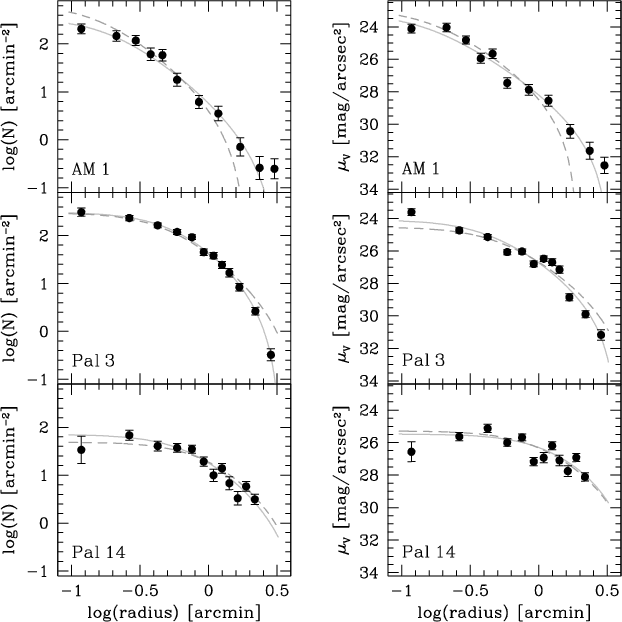
\includegraphics{figures/king-profiles.png}}
\end{center}

\begin{flushright}
Hilker (2005)
\end{flushright}

\vfill
\end{slide}


%------------------------------------------------------------------------------
\begin{slide}
\begin{center}
{\large \color{red} 
                  From $\rho$ to $f$  }
\end{center}

Given any functional form for $\rho(r)$ which is non-negative everywhere, it can be shown
that:
\eq{
	f(E) = \frac{1}{\sqrt{8}\pi^2} \frac{d}{dE} \int_E^0 d\Phi \frac{\rho'(\Phi)}{\sqrt{\Phi-E}}
}
where $\rho'(Phi) = d\rho(\Phi)/d\Phi$ and $\rho(\Phi)$ can be obtained by solving
the Poisson equation and inverting (see BT, Chapter~4, for details).

The above equation is useful in constructing isotropic models of spherical systems with
known density profiles (e.g., inferred from observations). In some cases,
these can be derived analytically (e.g., Jaffe 1983, or Henrquist 1990).

Generally, it can be solved numerically -- it's frequently used to set up
initial conditions for spherical systems in N-body calculations.

\vfill
\end{slide}



\end{document}


